\pagenumbering{arabic}
%\setcounter{page}{1}
\chapter{Introduction to R and Assessing Normality}
\index{Introduction}
\label{sec.matrix}
%start relabeling as 2.1 etc
\pagestyle{myheadings}  \markboth{\ref{sec.matrix}.
\titleref{sec.matrix}}{}
%\setcounter{equation}{0}

In this section, we will briefly introduce R, a useful tool for statistical computing and data visualisation, discuss quantitative data with its properties, basic statistical value calculation and box plot.\\

\section{Basic}

%\subsection{What is Statistics} \label{ssec.defm}\markright{\ref{ssec.defm} \titleref{ssec.defm}}

Intuitively, statistics can be considered the science of uncertainty. Formally,

\begin{definition}[Statistics]	\index{Statistics!Definition}
Statistics is the science of collecting, classifying, summarizing, analyzing and interpreting data.
\end{definition}

\section{What Is R?}

R is used for data manipulation, statistics, and graphics. It is made of: operations ($+$,$ -$, $<$) which is for calculations on vectors, arrays and matrices; a huge collection of functions; facilities for making unlimited types quality graphs; user contributed packages (sets of related functions); the ability to interface with procedures written in C, C+, or FORTRAN and to write additional primitives. R is also an open-source computing package which has seen a huge growth in popularity in the last few years (Please use this website: https://cran.r-project.org, to download R).
\\

\bigbreak

\noindent
\textbf{What is RStudio?}

RStudio is a relatively new editor specially targeted at R. RStudio is cross-platform, free and open-source software (Please use: https://www.rstudio.com, to download Rstudio).

\newpage

\section{Quantitative Data}

A common graphical representation of quantitative data is a histogram. This graphical summary can be prepared for data previously summarised in either a frequency, relative frequency, or percent frequency distribution. A histogram is constructed by placing the variables of interest on the horizontal axis and the frequency, relative frequency, or percent frequency on the vertical axis.
\\

\begin{itemize}
	\item Bar Charts v.s. Histograms: \\
	$1.$ Bar chats are for qualitative or categorical data (i.e. Favourite food data for 100 different students at UTM). \\
	$2.$ Histograms are for quantitative or numerical data (i.e. STA258 final mark from 100 different students at UTM).
\end{itemize}

\begin{itemize}
	\item Advantages of Histograms:\\
	$1.$ Histograms are easily to used for visualise data (relatively). It allows us to get the idea of the "shape" of distribution (i.e. skewness which will be discussed late in this section).\\
	$2.$ It is also flexible that people are able to modify bin widths.
	\item Disadvantages of Histograms:\\
	$1.$ It is not suitable for small data sets.\\
	$2.$ The values from histograms close to breaking points are likely similar, in fact they need to be classified into different bins (i.e. Student A and B scores 79 and 80 respectively in 		STA258, we consider a breaking point between 79 and 80. The two students have similar score, but student A is $B^+$ and student B is $A^-$ in GPA from).
	\item Skewness and Empirical Rule (or $68-95-99.7$ Rule):\\
		There are three types of skewness that are right (or positive) skewed (i.e. $\chi^{2}$ distribution), left (negative) skewed and symmetric. For any symmetric (bell-shaped) curve (i.e. normal distribution and $t-$ distribution), it follows the Empirical Rule as the following defined:
		\begin{definition}[The Empirical Rule (or $68-95-99.7$ Rule)]
		For any symmetric (bell-shaped) curve, let $\mu$ be its mean and $\sigma$ be its standard deviation, the following probability set function is true:
			\begin{itemize}
				\item  $1.$: $Pr(\mu - \sigma < X < \mu + \sigma) = 68.27\%;$
				\item  $2.$: $Pr(\mu - 2\sigma < X < \mu + 2\sigma) = 95.45\%;$
				\item  $3.$: $Pr(\mu - 3\sigma < X < \mu + 3\sigma) = 99.73\%.$
			\end{itemize}
		\end{definition}
		
\end{itemize}

% Need insert image(s) to demonstrate different types of skewness. (!!!!!!!!!!!!!)

\begin{figure}[H]
	\centering
	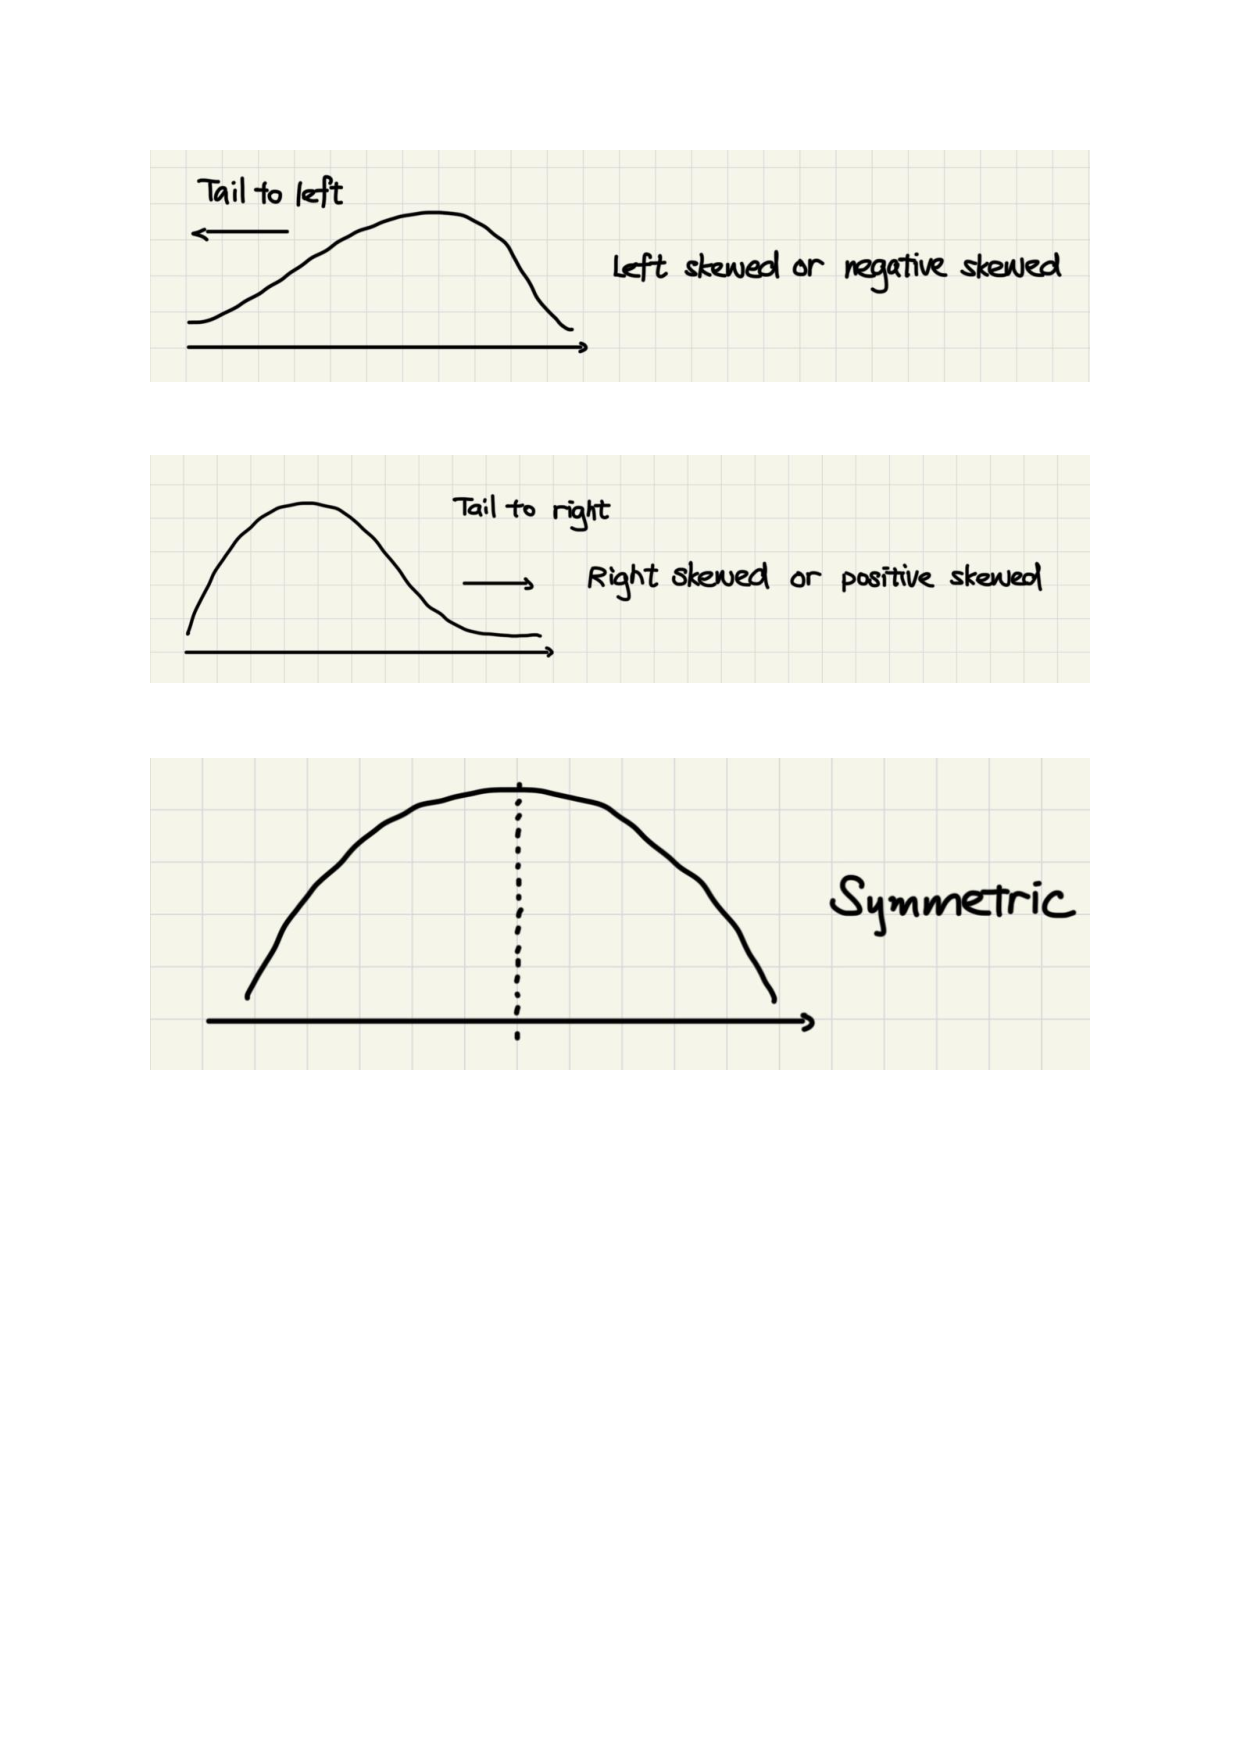
\includegraphics[scale=1.25]{Section1/img/SkewnessAll.pdf}
	\caption{Visualization of the a population, sample and a unit}
\end{figure}

\section{Basic Statistical Value Calculation:}

To begin with this section, we start from three main measures in quantitative statistics are the mean, variance and standard deviation. These measures form the basis of any statistical analysis.\\

\subsection{Sample Mean, Sample variance and Sample Standard Deviation}

%\begin{definition}
%	Let $x_1, x_2, x_3, ..., x_n$ be a sample of data points. We define sample mean of the sample data points ($\bar{x}$) as the following: \[ \bar{x} = \frac{1}{n} \sum_{i=1}^{n} x_i.\] Also, we define sample variance of the sample data points ($s^2$) as: \[ s^2 = \frac{1}{n-1} \sum_{i=1}^{n}(x_i - \bar{x})^2.\] Moreover, the standard deviation of the sample of data points ($s$) is: \[ s = \sqrt{s^2}, \quad \text{for } s > 0.\]
%\end{definition}

\begin{definition}
	Let $x_1, x_2, x_3, ..., x_n$ be a sample of data points. We define sample mean of the sample data points ($\bar{x}$) as the following: 
	$$ \bar{x} = \frac{1}{n} \sum_{i=1}^{n} x_i. $$
	Also, we define sample variance of the sample data points ($s^2$) as: \[ s^2 = \frac{1}{n-1} \sum_{i=1}^{n}(x_i - \bar{x})^2.\] Moreover, the standard deviation of the sample of data points ($s$) is: \[ s = \sqrt{s^2}, \quad \text{for } s > 0.\]
\end{definition}
	
\begin{example}
Let: $x_1 = 1, x_2 = 3$ and $x_3 = 7$. Calculate the sample mean, sample variance and sample standard deviation for this collection of data points.\\


Solution (all results are kept in four digits):\\
By Definition $1.2$, sample mean: \[ \bar{x} = \frac{1+3+7}{3} \approx 3.6667.\]
Then, we use sample mean to calculate sample variance: \[ s^2 = \frac{1}{3-1} \times [(1-3.6667)^2+(3-3.6667)^2+(7-3.6667)^2] \approx 9.3333.\]
Finally, we take the square root of sample variance to get sample deviation, and remember that $s > 0$: \[ s = \sqrt{s^2} \approx 3.0551.\]

\end{example}

\subsection{Median, Percentile and Quartile:}
	
Now, we move to median and percentile. Median indicates the information about the central value of a given collection of data points; percentile: $p^{th} \text{ percentile}$ which is a value that indicates $p \%$ of observations are below it.\\

\textbf{Median:}

\begin{definition}
Let: $x_1, x_2, x_3, ... , x_n$ be a collection of data points which is arranged in ascending order from the smallest value to the largest value (or descending order from the largest value to the smallest value in that collection). The median of the given collection of data points is the middle value in that collection, which equally spreads the collection into two parts. Half of all the collection values are above the median value and the rest of the values in the collection is below the median value.
\begin{itemize}
	\item Case 1: when n is an odd number. (i.e. $1, 3, 11, 237,...$). Then, the median $M$ is defined as: \[ M = \frac{n+1}{2} \text{, where n represents the $n^{th}$ position}.\]
	\item Case 2: when n is an even number (i.e. $2, 6, 100, 500,...$). Then, the median $M$ is: the average value of $\frac{n}{2}$'s and $\frac{n+2}{2}$'s position, where n represents the $n^{th}$ position.
	\end{itemize}
\end{definition}

\begin{example}
Given two distinct collections of data points: $S_1$ = $\{2, 4, 6\}$ and $S_2$ = $\{1, 5, 16, 28\}$. Calculate the median of both two sets.\\


Solution: \\

For $S_1$, since $n = 3$ which is an odd number, so by $Definition \text{ } 1.3$, $M_{S_1} = 4$. For $S_2$, $n = 4$ in this case, so that we need to calculate the average of $\frac{n}{2}$ and $\frac{n+1}{2}$. Then, \[ M_{S_2} = \frac{5+16}{2} = 10.5.\]
\end{example}

\textbf{Percentile and Quartile:}

\begin{definition}
Let: $x_1, x_2, ..., x_n$ be a collection of data points in either ascending order. Percentile is denoted as: $p^{th}$, which indicates $p \%$ of observations are below to a such value. Quartiles, are special cases of percentile which equally spread the collection of data into four parts. Each part contains $25\%$ of the entire collection. More specifically, we define quartiles as the following:
\begin{itemize}
	\item $Q_1$: the $25$ percentile (or $25^{th}$), which shows that $25\%$ of the data points are below the value $Q_1$.
	\item $Q_2$: the $50$ percentile (or $50^{th}$), which shows that $50\%$ of the data points are below the value $Q_2$.
	\item $Q_3$: the $75$ percentile (or $75^{th}$), which shows that $75\%$ of the data points are below the value $Q_3$.
	\item $Q_2$ is qual to median.
\end{itemize}
Moreover, we use $Q_3 - Q_1$ to calculate interquartile range (I.P.R), which shows the spread of the whole data set.
\end{definition}
	
\begin{example}
Consider the data set $S = $ $\{4, 25, 30, 30, 30, 32, 32, 35, 50, 50, 50, 55, 60, 74, 110\}$. Calculate its median and $Q_1$ ($25^{th}$).\\


Solution:\\

Simply counting the number of data points, $n = 15$, such that $M_{S}$ = $\frac{15 + 1}{2}$ = $8$. Thus, the $8^{th}$ value in the set which is $35$.\\

Since we know the median of this collection of data points, we just need to find the median of the lower half of this data, which is exactly going to be $25$ percentile ($25^{th}$). In the lower half of the given collection (all values below the median), $n_{lower} = 7$. By $Definition \text{ } 1.3$, then median of the lower half ($25^{th}$) is going to be: \[ 25^{th} = \frac{7+1}{2} = 4, \text{ the $4^{th}$ position in the data set}.\] Thus, $Q_1$ ($25^{th}$) $= 30$. To find $Q_3$ ($75^{th}$), apply the same strategy will guide you to find the correct answer, and we leave this as an exercise to you.

\end{example}
	
\section{Box Plot:}

It is a relatively simple visualisation of data used to determine skewness and potential outliers. 
	
% Need image
	
	
	
	
	





